\documentclass[8pt]{beamer}
%\mode<presentation>
\usepackage{../../Reports/notation}
\usepackage{ProjectPres}
\usepackage{Febimages}
%\title{}
%\setbeamercovered{transparent} 
\setbeamertemplate{navigation symbols}{} 
%\addtobeamertemplate{navigation symbols}{}{%
%    \usebeamerfont{footline}%
%    \usebeamercolor[fg]{footline}%
%    \hspace{1em}%
%    \insertframenumber/\inserttotalframenumber
%}

%\logo{} 
%\institute{University of Bath} 
\usebackgroundtemplate{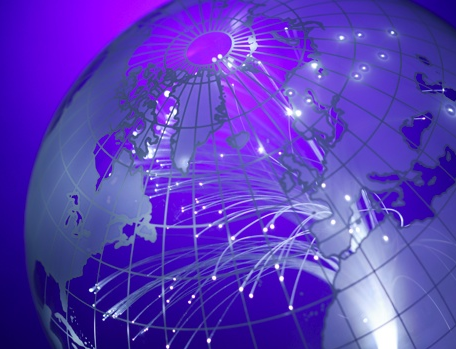
\includegraphics[width=\paperwidth,height=\paperheight]{PresImages/wifi.jpg}}
%\date{} 
%\subject{} 
\begin{document}

\begin{frame}
\begin{block}{}
\titlepage
\end{block}
\end{frame}

\begin{frame}
\begin{block}{Contents}
\tableofcontents
\end{block}

\end{frame}
\section{Introduction}
%------------------------------Introduction -0.5 minute -
% Introduction - Demand for wifi connection
%-Wifi in the homes. When did it start? 
%-Average number of devices in the past compared to now?
% Wireless communication was developed in 1960s with wifi developed in 1997.
%- 1998 saw the first wifi devices go into the home with 13% of homes having internet access. These homes would have had 1 device. Although internet access doesn't necessarily mean wifi an increase in the usage of the internet will increase the demand for wifi to be fast in order to keep up. Since this figure is low the need for speed was lower. 
%- In 2017 90% of homes have internet access with an average of 10 devices per home. Intel predict this to go up to 50 devices per home as the internet of things develops. As society becomes more dependent on internet connection there is user demand for connection to be fast. 
\begin{frame}{}
\vspace{-\parameterheight}
\begin{block}{Wireless communication}
\begin{minipage}{\threecols}
\desktop
\end{minipage}%
\begin{minipage}{\sepwid}
\mbox{}
\end{minipage}%
\begin{minipage}{\twocols}
\begin{multicols}{2}
% current speeds 2.4GHz and current number of devices. 
\phone
\tablet
\laptop
\smarttv
\end{multicols}
\end{minipage}
\pause 
\begin{minipage}{\threecols}
New technology
\begin{itemize}
\item Beam steering antennas.
\item Multi-Input-Multi-Output (MIMO).
\item \textbf{Ultra high frequency - (upto 60Ghz).}
\end{itemize}
\end{minipage}%
\begin{minipage}{\sepwid}
\mbox{}
\end{minipage}%
\begin{minipage}{\twocols}
\begin{multicols}{2}
\washingmachine
\IOT
\kettle
\fridge
\end{multicols}
\end{minipage}
\end{block}
\footnotetext{\footfullcite{desktop}}
\end{frame}
\newcommand{\Aims}{
\textbf{Optimise} the wireless \textbf{coverage} in the home. 
\par The homes can not be changed but the router \textbf{locations}, router \textbf{types}, \textbf{number} of interacting transmitters can all be chosen.
\par The optimal solution could use \textbf{antenna patterns (directivity)} that don't exist for existing technology but could be used to motivate future antenna developments.
\begin{itemize}
\item \textbf{Create an accurate and efficient model to simulate indoor-to-indoor WiFi and higher frequency (2.4GHz and upwards) wave propagation}.
\item \textbf{Use this model to optimise the quality of coverage in the home.} This requires maximising an appropriate quality function (to be chosen) by choosing the best:
\begin{itemize}
\item Antenna - Pattern and wavelength.
\item Antenna location and/or the location of multiple antennas.
\end{itemize}
\end{itemize}}
\begin{frame}{The Objective}
\begin{block}{The Aims}
\Aims
\begin{centering}
\begin{minipage}{0.15\linewidth}
\mbox{}
\end{minipage}%
\begin{minipage}{0.7\linewidth}
\plainroom
\end{minipage}
\end{centering}
\end{block}
\end{frame}

\begin{frame}{The Objective}

\begin{block}{The Aims}
\Aims
\begin{minipage}{0.15\linewidth}
\mbox{}
\end{minipage}%
\begin{minipage}{0.7\linewidth}
\Heatmap
\end{minipage}
\end{block}
\hspace{0.3\linewidth}
\end{frame}

\begin{frame}{The modelling problem -- Why high frequency?}
\vspace{-0.3cm}
\begin{block}{Frequency choice}
% Please add the following required packages to your document preamble:
% \usepackage{multirow}
\begin{table}[]
\begin{tabular}{|l|l|l|l|l|l|}
\hline
\multicolumn{3}{|l|}{f / GHz}                                     & \multicolumn{2}{l|}{pros}                                                                                              & cons                                                                                                       \\ \hline
\multirow{2}{*}{2.5} & \multicolumn{2}{l|}{\multirow{4}{*}{Wifi}} & \multirow{5}{*}{well understood}                                                   & \multirow{4}{*}{penetrates walls} & \multirow{4}{*}{\begin{tabular}[c]{@{}l@{}}narrow bandwidth\\ interference\\ less reflection\end{tabular}} \\
                     & \multicolumn{2}{l|}{}                      &                                                                                    &                                   &                                                                                                            \\ \cline{1-1}
\multirow{2}{*}{5}   & \multicolumn{2}{l|}{}                      &                                                                                    &                                   &                                                                                                            \\
                     & \multicolumn{2}{l|}{}                      &                                                                                    &                                   &                                                                                                            \\ \cline{1-3} \cline{5-6} 
3.4                  & \multirow{5}{*}{5G}   & 4G                 &                                                                                    &                                   & expensive                                                                                                  \\ \cline{1-1} \cline{3-6} 
\multirow{2}{*}{30}  &                       & \multirow{2}{*}{}  & \multirow{4}{*}{\begin{tabular}[c]{@{}l@{}}wide bandwidth\\ low cost\end{tabular}} & \multirow{2}{*}{reflects}         & \multirow{4}{*}{\begin{tabular}[c]{@{}l@{}}doesn't penetrate walls \\ still under study \\ susceptible to roughness \\ short range\end{tabular}}                                                                   \\
                     &                       &                    &                                                                                    &                                   &                                                                                                            \\ \cline{1-1} \cline{3-3} \cline{5-5}
\multirow{2}{*}{60}  &                       & \multirow{2}{*}{}  &                                                                                    & \multirow{2}{*}{}                 &                                                                                                            \\
                     &                       &                    &                                                                                    &                                   &                                                                                                            \\ \hline
\end{tabular}
\end{table}High frequency ($>$5 GHz) \textbf{coverage is good in one room} but doesn't travel well through walls. 
The model should be good for Wifi but becomes more accurate as the frequency gets higher.
\end{block}
\end{frame}
\begin{frame}{The modelling problem -- What is the domain?}
\begin{block}{Difficulties from the environment}
\begin{itemize}
\item The layout of lots of homes is unknown.
\item The exact physical composition of furniture and walls is not known.
\item Large variation between homes.
\end{itemize}
Because of these difficulties we aim to create a model which gives information about the coverage in the environment but do not expect exact results.
\par Our model currently takes the locations of objects as a user input but treats the physical parameters corresponding to those objects as unknown. 
\par \textit{Aim to use the probability of objects in locations at a later date.}
\end{block}
\end{frame}
\section{Mathematical formulation}
\begin{frame}{Mathematical problem}
\begin{block}{What is the mathematical aim of the project?}
Coverage Prediction:
\begin{itemize}
\item Estimating the electromagnetic field by approximating solutions to Maxwell's equations using the high frequency limit.
\item In free space %FIXME (insert free space definition)
 this is equivalent to estimating solutions to the Helmholtz equation.
\end{itemize}
It then remains to \textbf{optimise} the antenna pattern, wavelength and location. 
\par This requires choosing a suitable function which \textbf{quantifies the quality} of the coverage and then investigate suitable optimisation methods based on the structure of that function.
%  Wifi is an electromagnetic field. By trying to model wifi we are trying to evaluate this field everywhere. Since electromagnetic fields are modelled by Maxwells equations we are estimating solutions to these equations. 
% For known environments it is difficult to get exact solutions to these equations. There are numerical methods which estimate solutions but these become computationally expensive for high frequency.
% We don't know the boundary conditions since we don't know all the physical characteristics of the environment. Therefore even a computationally expensive method wouldn't be able to give us solutions.
% In free space Maxwells Equations are equivalent to the Helmholtz equations. The Helmholtz equation is also computationally difficult to get solutions to but using asymptotics we can formulate rays which represent wave fronts. These are what we use to estimate the field.
\end{block}
\end{frame}
\begin{frame}{Mathematics --- Maxwell's Equations}
\vspace{-0.3cm}
\begin{block}{}
\begin{subequations}
\begin{equation}
  - \pddt (\underbrace{\bD}_{\substack{\text{electric} \\ \text{flux} \\ \text{density}}} )+ \curl\underbrace{\bH}_{\substack{\text{magnetic} \\ \text{flux} \\ \text{density}}} = \underbrace{\bJ}_{\substack{\text{current} \\ \text{ density}}}      \  \text{ Maxwell Amp\`ere law}, \label{eqn::MaxwellAmpere3dlaw}
  \end{equation}
  \begin{equation}
   \pddt (\underbrace{\bB}_{\substack{\text{magnetic}\\ \text{field}}} )+ \curl \underbrace{\bE}_{\substack{\text{electric} \\ \text{field}}} =\pmb{ 0 }   \  \text{ Maxwell Faraday law}, \label{eqn::MaxwellFaraday3dlaw}
   \end{equation} 
   \begin{equation}
 \Div \bD = \underbrace{\rho}_{\substack{\text{charge} \\ \text{density}}}   \text{ Gauss electrical law} , \label{equan::Gausselectrical3dlaw}
 \end{equation}
 \begin{equation}
  \Div \bB = 0 \   \text{ Gauss magnetic law}, \label{eqn::Gaussmagnetic3dlaw}
\end{equation}
\label{eqn::Maxwell3D} 
\end{subequations}
Since the waves have single frequency $\freq$,
\begin{subequations}
\begin{equation}
\bE (\bx, t) = e^{i \freq t} \tilde{\bE}(\bx),
\end{equation}
\begin{equation}
\bB (\bx, t) = e^{i \freq t} \tilde{\bB}(\bx).
\end{equation}
\end{subequations}
\end{block}
\end{frame}
%- Propagation for monochromatic waves is modelled by Helmholtz equation.
%-Derive the high frequency approximation and therefore the eikonal equation.
% - phi is either the electric or magnetic field and we are interested in the field strength. 
% - u is the amplitude of phi and S is the path.
%- k is the wave number for ultra high frequencies this is very large.
\begin{frame}{Mathematical motivation}
\begin{block}{The Helmholtz equation}
The Helmholtz equation\footnotemark[1] models the electric ($\field=\bE$) or magnetic field ($\field=\bB$),
\begin{equation}
\lapla\field(x) +\wavenumber^2 \field(x) =0, \ \ k=\frac{\freq}{c}. \label{eqn::Helmholtzeqn}
\end{equation}
Approaches for solving:
\begin{itemize}
\item Finite Element Method
\item Finite Difference Time Domain
\item Finite Volume
\item Boundary Element Method 
\item \textbf{High frequency asymptotic approach - Ray method.} Many empirical methods are versions of ray methods.
\end{itemize}
\end{block}
\end{frame}
\begin{frame}{Mathematical motivation}
\begin{block}{Propagation model}
The Helmholtz equation\footnotemark[1] models the electric ($\field=\bE$) or magnetic field ($\field=\bB$),
\begin{subequations}
\begin{equation}
\lapla\field(x) +\wavenumber^2 \field(x) =0, \ \ k=\frac{\freq}{c}. \label{eqn::Helmholtzeqn}
\end{equation}
Use a WKB approximation and expand $\bu$ in powers for $\frac{i}{k}$
\begin{equation}
\field(x)=e^{i\wavenumber \phase(x)} \Big(\strength_0(\bx) +\frac{i}{\wavenumber} \strength_1(\bx)-\frac{1}{\wavenumber^2} \strength_2(\bx)+... \Big).
\end{equation}
\end{subequations}
The system of equations can then be written as,
\begin{subequations}
\begin{equation}
O(k^2): \ \ 1- |\nabla \phase (x)|^2=0, \ \ \text{The eikonal equation\footnotemark[2]} \label{eqn::Eikonal}
\end{equation}
\begin{equation}
O(k): \ \ \lapla \phase (\bx) \strength_0(\bx)+2 (\nabla \phase(\bx)\cdot\nabla)\strength_0(\bx)=\pmb{0}, \label{eqn::transportzero}
\end{equation}
\begin{equation}
O(k^{-m}): \ \ \lapla \strength_m(\bx)-(\lapla \phase(\bx)\strength_{m+1}(\bx)+2(\nabla \phase \cdot \nabla) \strength_{m+1}(\bx)))=\pmb{0}, \forall m \in  \mathbb{N}.
\end{equation}
\end{subequations}
\end{block}
\footnotetext[1]{\fullcite{cessenat1996mathematical}}
\footnotetext[2]{\fullcite{yun2015ray}}
\end{frame}
\begin{frame}{Ray theory}
\begin{minipage}{0.5\linewidth}
\begin{defn}[Wavefront]\label{defn::wavefront} \
The \textit{wavefronts $\wavefront(\bx)$} of a solution to the Helmholtz equation \eqref{eqn::Helmholtzeqn} with the form $\field (\bx) = \strength (\bx) e^{i \wavenumber \phase (\bx) }$, are the surfaces with 
$\phase(\bx)=constant$.
\end{defn}
\end{minipage}
\begin{minipage}{0.05\linewidth}
\mbox{}
\end{minipage}
\begin{minipage}{0.4\linewidth}
\begin{block}{} \wavefrontdiagram \vspace{-1cm} \end{block}
\end{minipage}
\begin{defn}[Ray]\label{defn::ray}
The \textit{rays} parameterised by $\charray$ corresponding to a wavefront $\wavefront(\bx(\charray))$, are the curves orthogonal to $\wavefront(\bx(\charray))$. \\ i.e. Let $\field (\bx) = \strength (\bx) e^{i \wavenumber \phase (\bx) }$ be a solution to the Helmholtz equation \eqref{eqn::Helmholtzeqn}, set $\propfac (\bx)$ to be an arbitrary proportionality factor. Then $\phase(\bx)$ and $\charray$ satisfy the orthogonality condition\footnote{This is for the three dimensional case. In $\dimension$ dimensions $\othersumvar=1,...,\dimension$.}:,
\begin{equation}
\label{eqn::rayorthogcond}
\frac{d x_\othersumvar}{d \charray}=\propfac (\bx) \frac{d \phase}{d x_\othersumvar}, \ \ \othersumvar=1,2,3. 
\end{equation}
\end{defn}
\end{frame}
\begin{frame}
\begin{block}{Straight rays}
Manipulation of the orthogonality condition gives,
\begin{equation}
\frac{d}{d \charray}\frac{1}{\propfac}\frac{d x_\othersumvar}{d \charray}= \frac{\propfac}{2} \frac{d}{d x_\othersumvar} \sum_{\sumvar=1}^3  \left(\frac{d \phase}{d x_\sumvar} \right)^2 .
\label{eqn::dsdxjsq}
\end{equation}
Using that $\phase(\bx)$ satisfies the eikonal equation and setting the proportionality factor to be 1,
\begin{equation}
\frac{d x_\othersumvar}{d \charray}= \constone.
\end{equation}
The equation for $x_\othersumvar$,
\begin{equation}
 x_\othersumvar= \constone\charray +\consttwo.
\end{equation}
The terms $\constone$ \& $\consttwo$ are constants. 
\end{block}
\end{frame}
\begin{frame}
\begin{block}{The strength on the ray}
To evaluate the strength on the ray use that $$ \grad \cdot \left( |\strength_0(\bx)|^2\grad \phase (\bx)\right)=|\strength_0(\bx)|^2\lapla \phase(\bx)+\grad\left(|\strength_0(\bx)|^2\right) \cdot \grad \phase(\bx).$$
Then rewrite the right-hand side,
$$ \grad \cdot \left( |\strength_0(\bx)|^2\grad \phase (\bx)\right)=\strength_0(\bx)^T\left(\strength_0(\bx)\lapla \phase(\bx)+2(\grad \phase(\bx)\cdot \grad)\strength_0(\bx)\right).$$
Since $\strength_0(\bx)$ satisfies the transport equation \eqref{eqn::transportzero} this is all zero.
\begin{equation}
\grad \cdot \left( |\strength_0(\bx)|^2\grad \phase (\bx)\right)=0
\end{equation}
\end{block}
\end{frame}
\begin{frame}
\begin{block}{}
\begin{minipage}{0.35\linewidth}
\wavefrontdiagram
\end{minipage}
\begin{minipage}{0.6\linewidth}
Integrate over a ray tube $F$,
\begin{equation}
\int_F \grad \cdot \left( |\strength_0(\bx)|^2\grad \phase (\bx)\right).dV=0.
\end{equation}
Then apply Gauss Theorem
\end{minipage}
\begin{equation}
0 =  \int_{\wavefront(\charray)} \left( |\strength_0(\charray') |^2\grad \phase (\charray') \right) \cdot \bn . dA(\charray')-  \int_{\wavefront(\charray_0)} \left( |\strength_0(\charray') |^2\grad \phase (\charray') \right)\cdot \bn . dA(\charray').
\label{eqn::applygauss}
\end{equation}
\pause
\par Since $(|\grad \phase |)^2=1$, $(\grad \phase \cdot \bn)^2=(|\grad \phase| )^2=1$, and therefore $\grad \phase \cdot \bn = \pm 1$. Substitute this into \eqref{eqn::applygauss} to get,
\begin{equation}
\int_{\wavefront(\charray)}  |\strength_0(\charray') |^2 .  dA(\charray')- \int_{\wavefront(\charray_0)}|\strength_0(\charray') |^2 . dA(\charray') =0.
\end{equation}

\end{block}
\end{frame}
\begin{frame}
\begin{block}{}
\par Since $|\strength_0|^2 $ is continuous on $\wavefront(\charray)$ we get,
\begin{equation}
|\strength_0(\charray) |^2 \delta A (\charray)=|\strength_0(\charray_0) |^2 \delta A (\charray_0).
\end{equation}
\par Rearrange this equation to get an expression for the field at $\charray$,
\begin{equation}
\strength_0(\charray)  =\strength_0(\charray_0)  \left(\frac{\delta A (\charray_0)}{\delta A (\charray)}\right)^{\frac{1}{2}}.\label{eqn::fieldzerofirst}
\end{equation}
\end{block}
\end{frame}
\begin{frame}
\begin{block}{The strength on the ray}
\begin{equation}
\strength_0 (\bx(\charray))= \strength_0 (\bx(\charray_0))\left(\frac{dA(\charray_0)}{dA(\charray)}\right)^{\frac{1}{2}}, \label{eqn::strengthzero}
\end{equation}
Define $\functwo(\charray)=\left(\frac{dA(\charray_0)}{dA(\charray)}\right)^{\frac{1}{2}}$. 
\begin{equation}
\strength_\sumvar (\bx(\charray))= \strength_\sumvar (\bx(\charray_0))\functwo(\charray)-\frac{1}{2} \int_{\charray_0}^\charray \frac{\functwo(\charray)}{ \functwo(\charray')}\lapla \strength_{\sumvar-1}. d \charray'.
\end{equation}
Therefore taking the approximation for $\wavenumber$ large $\strength \approx \strength _0$. 
\par This is similar to the Friis Transmission Equation. Set the gain of the transmitting antenna to be $G_T$ and the gain of the receiving antenna to be $G_R$, $\lambda$ to be the wavelength and $d$ the distance to the antenna. Then the power at the receiving antenna $\power_R$ in terms of the power from the source $\initpower$ is given by,
\begin{equation}
\power_R=\initpower G_T G_R \left( \frac{\lambda}{4 \pi  \rad}\right)^2.
\end{equation}
\end{block}
\end{frame}
\begin{frame}{Rays from conservation of power}
\begin{block}{Power}
\begin{minipage}{0.8\linewidth}
\begin{minipage}{0.4\linewidth}
\uniformpropagation %FIXME change isotropic antenna image
\end{minipage}
\begin{minipage}{0.15\linewidth}
\
\end{minipage}
\begin{minipage}{0.4\linewidth}
\raycone
\end{minipage}
\end{minipage}
\par Conservation of power means that for an isotropic antenna the total power over the surface of the sphere is the same as the power emitted from the point source. 
\end{block}
\end{frame}
\begin{frame}
\begin{block}{}
\par Assuming propagation is equal in all directions then the power 
on the surface of the cone $\conearea$ is $\power_A=\initpower\frac{4\pi \rad^2}{area(\conearea)}$. 
\par The power at any point in the cone is $\frac{\power_A}{area(\conearea)}$.
\end{block}
\begin{block}{}
\begin{minipage}{\linewidth}
\begin{minipage}{0.45\linewidth}
\rayconeDiscrete
\end{minipage}
\begin{minipage}{0.45\linewidth}
\par Tessellate the sphere with $\nrays$ number of cones. Then if each cone has equal size then $area(\conearea)=\frac{4 \pi \rad^2}{\nrays}$. 
\par Therefore the power at any point is $\frac{\initpower}{4\pi \rad^2}$. Power is proportional to the field squared, this agrees with equation \eqref{eqn::strengthzero}.
\par The power over the surface of each cone is $\frac{\initpower}{\nrays}$.
\par Accounting for the receiving aperture is $G_R \times \lambda^2$ and therefore we can estimate the receiving power at a point by the Friis transmission equation:
\begin{equation}
\power_R=\initpower G_T G_R \left( \frac{\lambda}{4 \pi  \rad}\right)^2.
\end{equation}
\end{minipage}
\end{minipage}
\end{block}
\end{frame}
\begin{frame}{Rays and obstacles}
%FIXME they do this so this needs to be more sophisticated and defined.
\begin{block}{Obstacle Interactions}
When a ray hits an object part of it is transmitted, part is reflected and sometimes part is scattered or diffracted.
\begin{minipage}{\linewidth}
\begin{minipage}{0.27\linewidth}
\rayeffectreflection \footnotemark[1]
\end{minipage}
\begin{minipage}{0.21\linewidth}
\rayeffectscattering  
\footnotemark[2]
\end{minipage}
\begin{minipage}{0.18\linewidth}
\rayeffecttransmission
\end{minipage}
\begin{minipage}{0.29\linewidth}
\rayeffectroughness \footnotemark[1]
\end{minipage}
\end{minipage}
\footnotetext[1]{\fullcite{aragon2008antennas}}
\footnotetext[2]{\fullcite{Keller62diffraction}}
\end{block}
\end{frame}
\begin{frame}{Ray Cones at reflection}
\begin{block}{Spreading loss after reflection}
\begin{minipage}{0.45\linewidth}
\standardcone
\end{minipage}
\begin{minipage}{0.45\linewidth}
\standardconetwo
\end{minipage}
\end{block}
\end{frame}
\begin{frame}{Field at reflection}
\vspace{-0.5cm}
\begin{block}{Field loss}
The amplitude of the field is proportional to square root of the power. %
\begin{minipage}{\twocols}
\begin{equation}
\power=Z_0^{-1}|E|^2
\end{equation}
\end{minipage}%
\begin{minipage}{\sepwid}
\mbox{}
\end{minipage}%
\begin{minipage}{\twocols}
\begin{equation}
\power=Z_0|B|^2
\end{equation}
\end{minipage}%
\\
\noindent\rule{\linewidth}{0.4pt}%
\\
\begin{minipage}{\twocols}
\vspace{-1cm}
Friis transmission equation \footnotemark[1]: \\
- \textbf{$\rad$ the distance} from the source to receiver, 
\\-  \textbf{$\lambda$ the wavelength},
\begin{equation*}
\underbrace{|\field_r|}_{\substack{\text{Field} \\ \text{strength} \\ \text{at} \\ \text{receiver}}}=\underbrace{|\field_0^*|}_{\substack{\text{Field} \\ \text{strength} \\ \text{emitted} \\ \text{at source}}}\sqrt{\underbrace{G_TG_R}_{\substack{\text{Gains} \\\text{of the} \\  \text{antennas}}}} \left(\frac{\lambda}{4 \pi \rad} \right).
\end{equation*}
\end{minipage}%
\begin{minipage}{\sepwid}
\mbox{}
\end{minipage}%
\begin{minipage}{\twocols}
Loss at reflection:
\\- The \textbf{Fresnel reflection coefficient\footnotemark[1]}, is a function of the \textbf{permittivity ($\epsilon$) and permeability ($\mu$)} of the mediums and the angle of incidence and transmission,
\begin{equation*}
\underbrace{\begin{bmatrix}
\field^{\text{ref}}_{||} \\ \field^{\text{ref}}_{\perp}
\end{bmatrix}}_{\substack{\text{Field strength} \\ \text{after reflection}}}=\underbrace{
\begin{bmatrix} \refcoef_{||} & 0 \\ 0 & \refcoef_{\perp}  \end{bmatrix}}_{\substack{\text{Fresnel} \\ \text{reflection} \\ \text{coefficient}}}\underbrace{\begin{bmatrix} \field^{\text{in}}_{||} \\ \field^{\text{in}}_{\perp}
\end{bmatrix}}_{\substack{\text{Field strength} \\ \text{into reflection}}}.
\end{equation*}
- The $\epsilon$ and $\mu$ parameters used to calculate $\refcoef_{||}$ and $\refcoef_{\perp}$ vary with frequency.
\end{minipage}
%\vertspace
\end{block}
\footnotetext[1]{\fullcite{aragon2008antennas}}
 \end{frame}
\begin{frame}{Ray-tracing theory}
\begin{block}{Field considering roughness}
There's also loss from interference of phase.
\\
\noindent\rule{\linewidth}{0.4pt}%
\\
\begin{minipage}{\twocols}
\vspace{-1cm} Friis transmission equation \footnotemark[1]: \\
- \textbf{$r$ the distance} from the source to receiver, 
\\-  \textbf{$\lambda$ the wavelength},
\begin{equation*}
\underbrace{\field_r}_{\substack{\text{Field} \\ \text{strength} \\ \text{at} \\ \text{receiver}}}=\underbrace{|\field_0^*|}_{\substack{\text{Field} \\ \text{strength} \\ \text{emitted} \\ \text{at source}}}\sqrt{\underbrace{G_TG_R}_{\substack{\text{Gains} \\\text{of the} \\  \text{antennas}}}} \left(\frac{\lambda}{4 \pi r} \right)e^{ikr}.
\end{equation*}
\end{minipage}%
\begin{minipage}{\sepwid}
\mbox{}
\end{minipage}
\begin{minipage}{\twocols}
Loss at reflection with a phase shift from roughness:
\begin{equation*}
\underbrace{\begin{bmatrix}
\field^{\text{ref}}_{||} \\ \field^{\text{ref}}_{\perp}
\end{bmatrix}}_{\substack{\text{Field strength} \\ \text{after reflection}}}=\underbrace{
\begin{bmatrix} \refcoef_{||} & 0 \\ 0 & \refcoef_{\perp}  \end{bmatrix}}_{\substack{\text{Fresnel} \\ \text{reflection} \\ \text{coefficient}}}\underbrace{\begin{bmatrix} \field^{\text{in}}_{||} \\ \field^{\text{in}}_{\perp}
\end{bmatrix}}_{\substack{\text{Field strength} \\ \text{into reflection}}}\tau.
\end{equation*}
The phase shift is dependent on depth of roughness ($\Delta \xi$), the angle of incidence ($\theta_i$) and the wavelength($\lambda$).$\tau=4 \pi \cos(\theta_i)\frac{\Delta \xi}{\lambda}$. 
\\ Since we don't know $\Delta \xi$ we model this as a uniformly distributed random variable.
\end{minipage}%
\end{block}
\footnotetext[1]{\fullcite{aragon2008antennas}}
\end{frame}
%\begin{frame}{}
%\begin{block}{Ray-launching summary}
%\begin{itemize}
%\item Rays describe the wave fronts and therefore the direction of travel of the wave. We use ray cones to model the spacing between the rays.
%\item The power at points along the ray is estimated using the Friis transmission equation.
%\begin{equation}
%\power_R=\initpower G_T G_R \left( \frac{\lambda}{4 \pi  \rad}\right)^2.
%\end{equation}
%\end{itemize}
%\end{block}
%\end{frame}
%---------------------------Ray-tracing theory - amplitude -3 minutes-
%- Eikonal equation motivates ray-tracing approach.
%- Loss is given by the Fresnel reflection coefficient and Friis transmission equation.
%- These equations come from conservation laws.
%-The gains are taken to be 1 for simplification in this model since the direction of the antenna's is not known.
%- The physical parameters are not known so R is fixed in the current model.
%%\subsection{Ray tracing theory amplitude}

\section{Implementation}
\begin{frame}{Ray-launching implementation}
\begin{block}{Standard methods}
\begin{itemize}
\item Input all information about the environment.
\item Calculate reflection points
\item Iterate along each ray calculating the field.
\item Convert field values to power.
\item Output grid corresponding to power over the environment.
\end{itemize}
Repeat the entire process to get results for any variation of inputs.
\end{block}
\begin{block}{New approach}
\begin{itemize}
\item Input only the geographical information.
\item Calculate the reflection points.
\item Iterate through rays storing the information needed to later calculate the field in relevant positions.
\item Output grid of matrices containing the information needed to calculate the field.
\end{itemize}
The same output grid can be used to compute power grids corresponding to different inputs.
\end{block}
\end{frame}
\begin{frame}{Ray-launching}
\begin{block}{Trajectories}
\raysroom
\end{block}
\end{frame}
\begin{frame}{Ray-launching}
\begin{block}{Storing ray history}
\begin{minipage}{0.44\linewidth}
Discretise the environment into $\nx$, $\ny$, and $\nz$ pieces in the $x,y$ and $z$ directions.
\threedgrid
\end{minipage}%
\begin{minipage}{\sepwid}
\mbox{}
\end{minipage}%
\begin{minipage}{0.54\linewidth}
\pause
Each term in the mesh corresponds to a $(\nrefs*\nrays+1)\times (\nob *\nrefs+1)$ sparse matrix.
\begin{align*}
& \element= \\
& \begin{array}{l l}
\begin{array}{c c c c c}
\scriptscriptstyle{0} & \scriptscriptstyle{\cdots} & \scriptscriptstyle{\nrefs} & \scriptscriptstyle{\cdots} & \scriptscriptstyle{\nrefs*\nrays}
 \end{array} &
 \\
 \left(
\begin{array}{c c c c c}
 \ddots & \cdots &  & \cdots & \reflectbox{$\ddots$} 
 \\
\vdots & &  & & \vdots  \\
\vdots & &  & & \vdots \\
\reflectbox{$\ddots$} & \cdots & &  \cdots & \ddots 
\end{array}
 \right)
    & 
    \begin{array}{l}
    \scriptscriptstyle{0} \\ \vdots \\ \scriptscriptstyle{\nob}  \\ \vdots \\ \scriptscriptstyle{\nob*\nrefs}
  \end{array} \\
  \end{array}
\end{align*}
Each term in this matrix corresponds to a possible ray ($\nrays$), obstacle ($\nob$) interaction after $\nrefs$ reflections.
\end{minipage}
\\
\noindent\rule{\linewidth}{0.4pt}%
\\
\pause
\par Storage requirement: $\nx \times \ny \times \nz$, sparse matrices with dimension: $(\nrefs*\nrays+1)\times (\nob *\nrefs+1)$ with complex entries. Standard method requires $\nx \times \ny \times \nz$ complex terms.
\end{block}
\end{frame}
\begin{frame}{Single ray}
\begin{block}{Iterating through a ray and the cones}
\begin{multicols}{2}
\triangleonmesh
\vspace{-0.5cm}
\begin{itemize}
\item Compute a set normal vectors to the ray. 
\item Step along the ray and store the \textbf{ray history} in the element.
\item Determine No. of steps needed to reach the edge of the cone. 
\[
\text{integer}\left(\meshwidth^{-1}\edgelength\right)
\]
\item Step out along these normals storing the same history to these elements.
\item Move to the next step along the ray.
\item Repeat until the end of the ray segment.
\end{itemize}
\end{multicols}
\pause
At each stage check if the square is the same as the previous, if so move to the next step. 
\par In the cone check if the step's \textbf{inside an obstacle}, if so move to the next step.
\par
There is an error from stepping along the normal \textbf{rather than the curve} of the sphere but this distance error should be less than the size of one mesh square.
\end{block}
\end{frame}
\begin{frame}
\begin{block}{Storing the ray history}
\par The temporary vector $\pmb{v}$ is initialised as empty with datatype complex and length $\nob *\nrefs +1$.
\par When a ray hits obstacle number $n_{Ob}$ with angle $\theta_i$ after $n_{Re}\geq 1$ reflections the term $(e^{j\theta_i})$\footnotemark[1] is put in the row $\underbrace{\nob}_{\substack{\text{Total number} \\ \text{of obstacles}}}*\left(n_{Re}-1\right)+n_{ob}$ of the temporary vector $\pmb{v}$. 
\pause If $n_{Re}=0$ (i.e line of sight) then $1$ is put in the $1^{st}$ row but is removed before the next reflection.
\begin{minipage}{0.4\linewidth}
\[\pmb{v}=  \begin{array}{ll}
\begin{array}{l}
    \scriptstyle{0} \\ \vdots \\ \scriptscriptstyle{\nob*(n_{Re}-1)+n_{ob}}  \\ \vdots \\ \scriptscriptstyle{\nob*\nrefs}
  \end{array} 
  & \left( \begin{array}{l}
    \vdots \\ \\ e^{j\theta_i}  \\  \\ \vdots \\
  \end{array} \right)
  \end{array} \]
\end{minipage}%
\begin{minipage}{\sepwid}
\mbox{}
\end{minipage}%
\begin{minipage}{0.5\linewidth}
\pause
This vector $\pmb{v}$ is multiplied by the distance the ray has traveled and then stored in column $\underbrace{\nrefs}_{\substack{\text{Maximum}\\ \text{number} \\ \text{of reflections}}}*\underbrace{n_{Ra}}_{\substack{\text{current ray} \\ \text{number}}}+n_{Re}$ in the mesh element the ray has gone through\footnotemark[2].
\end{minipage}
\footnotetext[1]{$j$ is the imaginary number used instead of $i$ as not to confuse with the incidence angle.}
\footnotetext[2]{ray number counts from $0$ where as reflections start counting at $1$. Since the $0$ reflection can not correspond to any obstacle.}
\end{block}
\end{frame}
\begin{frame}
\begin{block}{Output}
\begin{minipage}{0.4\linewidth}
\threedgrid
\end{minipage}%
\begin{minipage}{\sepwid}
\mbox{}
\end{minipage}%
\begin{minipage}{0.52\linewidth}
\begin{align*}
& \element= \\
& \begin{array}{l l}
\begin{array}{c c c c c}
\scriptstyle{0} & \cdots & \scriptscriptstyle{\nrefs*n_{Ra}+n_{Re}} & \cdots & \scriptscriptstyle{\nrefs*\nrays}
 \end{array} &
 \\
 \left(
\begin{array}{c c c c c c c}
 \ddots & & & & & & \reflectbox{$\ddots$} \\
 & & \vdots & & & & \\ 
 \\ & \cdots & \rad e^{j\theta_i} & \cdots & & &  \\ & & \vdots & & & & \\
 \reflectbox{$\ddots$} & & & & & & \ddots 
\end{array}
 \right)
    & 
    \begin{array}{l}
    \scriptstyle{0} \\ \\ \vdots \\ \scriptscriptstyle{\nob*n_{Re}+n_{ob}}  \\ \\ \vdots \\ \scriptscriptstyle{\nob*\nrefs}
  \end{array} \\
  \end{array}
\end{align*} 
\end{minipage}
\par If $n_{Re}>0$ the column $\nrefs*n_{Ra}+n_{Re}$ must be either empty or contain $n_{Re}$ terms. \par If $n_{Re}=0$ (i.e line of sight path) then then column is either empty or contains $1$ term in the first row.
\end{block}
\end{frame}
\begin{frame}
\begin{block}{Power calculation}
To calculate the field from the mesh, input: \textbf{frequency, antenna gains, permittivity and permeability}.
\begin{itemize}
\item Retrieve the mesh of incidence angles.
\item Compute the mesh of \textbf{reflection coefficients} using the Fresnel reflection formula, the incidence angles and the refractive index of the obstacles (function of permittivity and permeability).
\pause 
\item Take the product of each column.
\item Multiply each column by the gains corresponding the that ray and the free space loss term: $|\field_0^*|\sqrt{\transgain \recgain}\left(\frac{\lambda}{4 \pi\rad}\right)e^{i\wavenumber\rad}$
\item Sum each column.
\pause
\item Output mesh of size $\nx\times \ny \times \nz$ containing complex values corresponding to the field.
\item Convert to power using $\power=Z_0^{-1}|E|^2=Z_0|B|^2$.
\end{itemize}
\end{block}
\end{frame}
\begin{frame}{Ray-launching}
\begin{block}{Power approximations - 2D Slice}
\Heatmap
\begin{itemize}
\item
The power can be calculated from the mesh and represented using a heatmap.
\item There is a loss in power as a result of the distance travelled and from the collisions.
\end{itemize}
\end{block}
\end{frame}
\begin{frame}
\begin{block}{Storing ray history - Summary}
\begin{itemize}
\item
The sparse matrix for each grid point \textbf{stores the angles the objects} have been hit at and the \textbf{distance the ray traveled} when it reached that grid point. 
\pause
\item 
The location of the term in the matrix corresponds to the \textbf{ray number, the reflection number, and the obstacle number}. 
\pause
\item Knowing the ray number allows us to change the \textbf{directivity} of the antenna.
\pause
\item Knowing the obstacle number allows us to change the \textbf{material} of the obstacle.
\pause
\item Knowing the reflection number allows us to distinguish between different collisions with the same obstacle.
\end{itemize}
\end{block}
\end{frame}

\begin{frame}{Comparison}
\begin{block}{Storing information vs storing field}
\begin{itemize}
\item The same number of steps needs to be made in both cases. However our main program only needs to be \textbf{run once} to get results corresponding to \textbf{multiple different parameter inputs}.
\pause
\item By storing the information we have the \textbf{function for the field} at each grid point rather than the value for one case. This will allow us to compute the sensitivity to different obstacles.
\pause
\item When optimising we can compute the quality function straight from the mesh without computing the field and power first.
\pause
\item The method is very compatible with parallelisation. \textbf{Each ray can be considered independently and then merged together}. 
\pause
\item One extra run can be done for an additional antenna location and the results can be used for considering \textbf{both antenna's together and comparison of each on their own}.
\pause 
\item The memory requirements are larger but not large enough to be a problem in a domestic environment.
\end{itemize}
\end{block}
\end{frame}
\section{Future work}
\begin{frame}{Future work -- Quality function}
\begin{block}{}
\begin{equation}
\quality=-\weightone \int_{\domain}\underbrace{ \spatialvar}_{\text{Spatial variation}}d\domain + \weighttwo\underbrace{ \covvalue}_{\text{Coverage value}} -\weightthree \int_{\domain}\underbrace{ \interf}_{Interference} d \domain
\end{equation}
MIMO technology accounts for spatial variation problems so $\weightone=0$.
\begin{equation}
\quality= \weighttwo\underbrace{ \covvalue}_{\text{Coverage value}} -\weightthree \int_{\domain}\underbrace{ \interf}_{Interference} d \domain
\end{equation}
The coverage value could be considered in different ways. Possible options: $\covvalue=$
\begin{multicols}{2}
\begin{itemize}
\item  $\int_{\domain} h_2(\domain)|\field|^2 d\domain$ --- weighted by user area
\item  $\max{|\field|_{a}}$ --- user in specific location
\item  $ \min{|\field|}$ --- least poor coverage
\item  $\max{|\field|_{\domain}}$ --- user in one location to be decided by optimisation.
\item $\int_{\domain} |\field|^2  d\domain $ --- average 
\end{itemize}
\end{multicols}
The structure of this quality function will determine the type of optimisation method.
\par Optimise after one run of the algorithm:
\begin{multicols}{2}
\begin{itemize}
\item wavelength
\item antenna pattern (gains)
\end{itemize}
\end{multicols}
It then remains to optimise the antenna location
by either running the algorithm many times or investigating further approaches.
\end{block}
\end{frame}
\begin{frame}{Future work}
\begin{block}{Sensitivity analysis}
From the main program for each element we have the function for the field,
\begin{equation}
\field_{x,y,z}=|\field_0^*|\sum_{k=0}^{\nrays}\sqrt{\transgain_{k} \recgain_{k}}\left(\frac{\lambda}{4\pi \rad_{k}}\right)e^{i \wavenumber \rad}\prod_{l=0,\refcoef\neq0}^{\nrefs}\refcoef_{\nob,\theta_i}.
\end{equation}
From this we then want to consider $\frac{\partial \field}{\partial \refcoef_{\nob}}$ to evaluate whether coverage would be good if a particular obstacle was lossy.
\end{block}
\end{frame}
\begin{frame}{Future work}
\begin{block}{Next steps}
\begin{itemize}
\item Make the method compatible with 3D visualisation software to view the power results.
\item Define the optimisation algorithm for choosing the antenna directivity and wavelength.
\item Investigate optimisation method for antenna location.
\item Build in interference model.
\end{itemize}
\end{block}
\end{frame}
\begin{frame}{Future work -- Impact}
\begin{block}{How will the results impact the industry?}
The results from the opimisation can be used for the following:
\begin{itemize}
\item \textbf{Recommending the correct device} for different home types.
\item \textbf{Informing engineers} as to which type of antennas would be worth researching. i.e what wavelengths and antenna patterns should they try and build.
\begin{itemize}
\item This could also be applied to optimal location. Should they try to build routers which attach to ceiling or walls?
\end{itemize}
\item Choose the \textbf{best antenna from the existing available equipment} and recommend the best location for coverage.
\end{itemize}
\end{block}
\pause
\begin{block}{}
Thank you.
\end{block}
\end{frame}

\begin{frame}{Appendix slides}
\end{frame}

\begin{frame}{Multi-dimensional sparse array}
\begin{block}{}
\begin{minipage}{0.8\linewidth}
\DictionarySparse
\end{minipage}
\begin{minipage}{0.17\linewidth}
\begin{itemize}
\item
\textbf{$nx, ny, nz$} --- number of grid points in the x, y and z axis.
\item \textbf{$na, nb$} --- number of rows and columns in each sparse matrix.
\end{itemize}
\end{minipage}
This class allows indexing similar to multidimensional numpy arrays \textbf{$ds[x,y,z,a,b]$} but uses a dictionary look up to a sparse matrix then indexes within the matrix.
\end{block}

\end{frame}

\begin{frame}{Reflection function}
\begin{block}{}
\begin{multicols}{2}
A ray is input to the reflection function as two points,
\begin{equation*}
\text{Ray}=(\underbrace{P_1}_{\substack{\text{Intersection}\\ \text{point}}},\underbrace{P_0}_{\substack{\text{Previous ray}\\  \text{intersection} \\ \text{point or} \\ \text{start}}}).
\end{equation*}
The triangle which the ray is being reflected with is three points,
\begin{equation*}
T=(T_0,T_1,T_2).
\end{equation*}
Translate the ray so that the intersection is the origin,
\begin{equation*}
\text{Ray}=(0,P_0-P_1).
\end{equation*}
Compute two edges of the triangle,
\begin{align*}
& e_0=T_0-T_1, \\
& e_1=T_0-T_2.
\end{align*}
Compute the normal to the triangle,
\begin{equation*}
n=(e_0 \times e_1)/ (||e_0 \times e_1||).
\end{equation*}
The image point is the same as the direction of the ray since the intersection was translated to the origin,
\begin{equation}
\text{Image}=(P_1-P_0)/(||P_1-P0||).
\end{equation}
Find the reflection point,
\begin{equation}
P_{Re}=\text{Image}-2(\text{Image} \cdot n) n.
\end{equation}
The reflected ray segment is : $(P_{Re}+P_1,P1)$
\end{multicols}
\end{block}
\end{frame}
\begin{frame}{Ray launcher}
\begin{block}{Inside or outside?}
\begin{itemize}
\item The points in the domain do not know which medium they are.
\item The reflection function always stops a ray when it hits an object so none of the points inside the objects get given a value.
\item When the cones are found there are values assigned to inside objects.
\item It is possible to stop this by running an intersection function at every step but this is very expensive given the number of steps along the ray and the number of rays.
\item Remove at the end.
\end{itemize}
\end{block}
\end{frame}
\begin{frame}{Computations}
\begin{block}{Maximum number of computations}
Excluding the input steps.
\begin{equation}
\sqrt{\nrays} \times \nrefs \times \left(\frac{\maxleng}{\meshwidth}\right)^2 \times
\sum_{n_{Re}=0}^{\nrefs}\left(4 \sqrt{\pi \left(2 \sqrt{2}n_{Re}\sin\left(\rayangle\right)\maxleng+\meshwidth \right)} \right)
\end{equation}
\end{block}
\end{frame}
\end{document}